\documentclass{article}
\usepackage[english,russian]{babel}
\usepackage{textcomp}
\usepackage{geometry}
  \geometry{left=2cm}
  \geometry{right=1.5cm}
  \geometry{top=1.5cm}
  \geometry{bottom=2cm}
\usepackage{tikz}
\usepackage{multicol}
\usepackage{hyperref}
\usepackage{listings}
\usepackage{pmboxdraw}
\usepackage{fancyvrb}
\pagenumbering{gobble}

\lstdefinestyle{csMiptCppStyle}{
  language=C++,
  basicstyle=\linespread{1.1}\ttfamily,
  columns=fixed,
  fontadjust=true,
  basewidth=0.5em,
  keywordstyle=\color{blue}\bfseries,
  commentstyle=\color{gray},
  texcl=true,
  stringstyle=\ttfamily\color{orange!50!black},
  showstringspaces=false,
  numbersep=5pt,
  numberstyle=\tiny\color{black},
  numberfirstline=true,
  stepnumber=1,      
  numbersep=10pt,
  backgroundcolor=\color{white},
  showstringspaces=false,
  captionpos=b,
  breaklines=true
  breakatwhitespace=true,
  xleftmargin=.2in,
  extendedchars=\true,
  keepspaces = true,
  tabsize=4,
  upquote=true,
}


\lstdefinestyle{csMiptCppLinesStyle}{
  style=csMiptCppStyle,
  frame=lines,
}

\lstdefinestyle{csMiptCppBorderStyle}{
  style=csMiptCppStyle,
  framexleftmargin=5mm, 
  frame=shadowbox, 
  rulesepcolor=\color{gray}
}

\lstset{style=csMiptCppStyle}
\lstset{literate={~}{{\raisebox{0.5ex}{\texttildelow}}}{1}}


\renewcommand{\thesection}{\arabic{section}}
\makeatletter
\def\@seccntformat#1{\@ifundefined{#1@cntformat}%
   {\csname the#1\endcsname\quad}%    default
   {\csname #1@cntformat\endcsname}}% enable individual control
\newcommand\section@cntformat{Часть \thesection:\space}
\makeatother



\begin{document}
\title{Семинар \#1: Подключение библиотек. Библиотека raylib.\vspace{-5ex}}\date{}\maketitle


\section{Библиотеки в языках C и C++}
\textbf{Библиотека в программировании} -- это набор готовых функций, классов или модулей(файлов), которые можно подключить к программе и использовать повторно для выполнения типовых задач.

В языках программирования C и C++ библиотеки можно разделить на следующие типы:
\begin{center}
\includegraphics[scale=0.86]{../images/libtax.pdf}
\end{center}
Разные типы библиотек создаются имеют свои особенности из создания и подключения. Для простоты будем предполагать, что мы используем язык C++ и компиляторы gcc и MinGW. Подключение библиотек на языке C и на других компиляторах во многом аналогично и отличается несущественно.

\begin{enumerate}
\item \textbf{Header-only библиотеки}\\
Самый простой тип библиотек. Весь их код размещается в заголовочных файлах (\texttt{.h}/\texttt{.hpp}) и подключается с помощью директивы \texttt{\#include}. Такие библиотеки легко использовать — как правило, достаточно добавить одну директиву \texttt{\#include}. Их основной недостаток заключается в том, что код библиотеки компилируется отдельно для каждого \texttt{.cpp} файла, в который она подключена, что может увеличить время компиляции.


\item \textbf{Раздельно компилируемый исходный код}\\
Библиотека представляет собой набор из заголовочных файлов(\texttt{.h}/\texttt{.hpp}) и файлов исходного кода(\texttt{.cpp}). Для подключения такой библиотеки вам нужно:
\vspace{-1mm}
\begin{itemize}
\item Добавить в код вашей программы необходимые заголовочные файлы, используя \texttt{\#include}.
\item Указать компилятору пути до всех \texttt{.cpp} файлов библиотеки в дополнении ко всем файлам программы.
\end{itemize}
\vspace{-1mm}
Однако, такой способ подключения практически не используется, так как одна библиотека может содержать огромное количество \texttt{.cpp} файлов и подключение их всех может быть неудобным. Вместо этого, разработчики библиотеки предоставляют специальные сценарии (например, для программ \texttt{make} или \texttt{CMake}), используя которые вы можете скомпилировать библиотеку и превратить её в статическую или динамическую библиотеку.


\item \textbf{Статическая библиотека}\\
Библиотека представляет собой набор из заголовочных файлов(\texttt{.h}/\texttt{.hpp}) и файлов скомпилированного кода статической библиотеки, которые имеют расширения:
\vspace{-1mm}
\begin{itemize}
\item \texttt{.a} -- на Linux, macOS, Windows(компиляторы MinGW и Clang); \texttt{.a} от слова archive
\item \texttt{.lib} -- на Windows(компилятор MSVC)
\end{itemize}
\vspace{-1mm}
Также, как правило, названия таких файлов начинаются с \texttt{lib}. К примеру, если у нас есть простая статическая библиотека по имени \texttt{dog}, то она будет состоять минимум из двух файлов:
\vspace{-1mm}
\begin{itemize}
\item \texttt{dog.hpp}
\item \texttt{libdog.a}
\end{itemize}
\vspace{-1mm}

Для подключения статической библиотеки к вашей программе вам нужно:
\begin{itemize}
\item Добавить в код вашей программы необходимые заголовочные файлы, используя \texttt{\#include}.
\item Указать компилятору путь до директории, содержащей заголовочные файлы, используя опцию \texttt{-I}.
\item Указать компилятору путь до директории, содержащей файлы скомпилированного кода, используя опцию \texttt{-L}.
\item Указать компилятору имя конкретного файла скомпилированного кода, используя опцию \texttt{-l}. При этом указывать приставку \texttt{lib} и расширение файла не нужно.
\end{itemize}
К примеру, если вы хотите подключить к вашей программе, состоящей из одного файла \texttt{main.cpp}, простую статическую библиотеку \texttt{dog}, упомянутую выше, то вам нужно сделать следующее:
\begin{itemize}
\item Добавить в начало вашего кода строку:
\begin{lstlisting}
#include "dog.hpp"
\end{lstlisting}
\item Скомпилировать программу со следующими опциями:
\begin{lstlisting}
$ g++ main.cpp -I <include directory> -L <lib directory> -l dog
\end{lstlisting}
где 
\begin{itemize}
\item \texttt{<include directory>} -- путь до директории, содержащей файл \texttt{dog.hpp}.
\item \texttt{<lib directory>} -- путь до директории, содержащей файл \texttt{libdog.a}.
\end{itemize}
При этом пробел между опцией и аргументом обычно опускают, то есть пишут \texttt{-ldog}, а не \texttt{-l dog}.

\end{itemize}

\item \textbf{Динамическая библиотека}\\
Библиотека представляет собой набор из заголовочных файлов(\texttt{.h}/\texttt{.hpp}) и файлов скомпилированного кода динамической библиотеки, которые имеют расширения:
\vspace{-1mm}
\begin{itemize}
\item \texttt{.so} -- на Linux; \texttt{.so} от shared object
\item \texttt{.dll} -- на Windows; \texttt{.dll} от dynamic link library
\item \texttt{.dylib} -- на macOS; \texttt{.dylib} от dynamic library
\end{itemize}
\vspace{-1mm}
Названия таких файлов на Linux имеет приставку \texttt{lib}, а на Windows и macOS такой приставки нет. Также на Windows вместе с динамической библиотекой \texttt{.dll} обычно поставляется небольшая библиотека \texttt{.a} или \texttt{.lib}, которая используется для подключения этой динамической библиотеки.

К примеру, если у нас есть простая динамическая библиотека на Lunux по имени \texttt{dog}, то она будет состоять минимум из двух файлов:
\vspace{-1mm}
\begin{itemize}
\item \texttt{dog.hpp}
\item \texttt{libdog.so}
\end{itemize}
\vspace{-1mm}
А на Windows такая библиотека будет обычно состоять из трёх файлов:
\vspace{-1mm}
\begin{itemize}
\item \texttt{dog.hpp}
\item \texttt{dog.dll}
\item \texttt{libdog.a} или \texttt{libdog.lib}
\end{itemize}
\vspace{-1mm}
Подключить динамическую библиотеку к вашей программе можно таким же образом, что и статическую.
\end{enumerate}

\subsection*{Отличие динамических библиотек от статических}
Основное отличие динамической библиотеки от статической заключается в том, что статическая библиотека встраивается в исполняемый файл на этапе компиляции, а динамическая библиотека загружается и подключается во время запуска программы. Такой подход имеет следующие преимущества:
\begin{itemize}
\item Статическая библиотека встраивается в итоговый исполняемый файл и увеличивает его размер, динамическая библиотека подключается только при запуске и не увеличивает размер исполняемого файла.
\item Одна и та же динамическая библиотека может быть загружена в память только один раз и использована сразу несколькими программами, что экономит оперативную память.
\item Динамическую библиотеку можно загружать и выгружать во время работы программы.
\end{itemize}
Недостаток динамических библиотек заключается в том, что для запуска программы, использующей их, необходимые библиотеки должны быть заранее установлены в системе. При их отсутствии программа не сможет запуститься.
\section{Создание и подключение библиотек}
Рассмотрим создание простой собственной библиотеки, используя все четыре её типа. Пусть имеется
следующая программа, содержащая функцию \texttt{cube}:
\begin{center}
\includegraphics[scale=1]{../images/00main_cube.pdf}
\end{center}
Вынесем функцию \texttt{cube} в отдельный файл и создадим простейшую библиотеку с одной функцией.
Разумеется, на практике библиотеки состоят из множества файлов исходного кода, каждый из которых
содержит множество функций. Здесь же мы создаём минимальный пример в учебных целях.

\subsection*{Создание и подключение header-only библиотеки}
Создать такую библиотеку очень просто --- достаточно вывести функцию в отдельный заголовочный файл.
\begin{center}
\includegraphics[scale=1]{../images/01main_cube_include.pdf}
\end{center}
После этого файл \texttt{cube.hpp} можно считать header-only библиотекой. Для подключения такой библиотеки достаточно просто добавить одну директиву \texttt{\#include} в файл исходного кода, где эта библиотека требуется. Чтобы скомпилировать программу, нужно просто написать:
\begin{lstlisting}
$ g++ main.cpp
\end{lstlisting}
Указывать файл \texttt{cube.hpp} для компилятора не нужно, так как он сам вставит этот файл внутрь файла \texttt{main.cpp} благодаря директиве \texttt{\#include}.

Ключевое слово \texttt{static} используется для предотвращения ошибок компоновки при подключении заголовка в нескольких файлах. Если не указать \texttt{static} перед функцией, то в программе из нескольких файлов при подключении заголовка как минимум к двум \texttt{.cpp} файлам возникнет ошибка множественного определения функции. При использовании \texttt{static} функция будет видна только в пределах одного .cpp файла, поэтому каждый \texttt{.cpp} файл получит собственную реализацию \texttt{cube}, и ошибка не возникнет. Альтернативой является использование ключевого слова \texttt{inline}.
 
 
\subsection*{Создание и подключение библиотек раздельно-компилируемого кода}
Используем раздельную компиляцию:
\begin{center}
\includegraphics[scale=1]{../images/02main_cube_separate.pdf}
\end{center}
Совокупность файлов \texttt{cube.hpp} и \texttt{cube.cpp} можно рассматривать как библиотеку. Для подключения такой библиотеки к файлу \texttt{main.cpp} нужно сделать следующее:
\vspace{-1mm}
\begin{enumerate}
\item Подключить заголовочный файл \texttt{cube.hpp} с помощью \texttt{\#include}.
\item Указать файл исходного кода \texttt{cube.cpp} при компиляции:
\begin{lstlisting}
$ g++ main.cpp cube.cpp
\end{lstlisting}
\end{enumerate}
\vspace{-1mm}
Недостатки такого подхода проявляются, если библиотека содержит не один, а множество файлов исходного
кода -- иногда сотни или даже тысячи. В этом случае:
\begin{itemize}
\item Может показаться, что потребуется подключать много заголовочных файлов, однако этого можно избежать,
создав один общий заголовок, который включает все необходимые файлы.
\item При компиляции нужно будет указывать все \texttt{.cpp} файлы библиотеки.
\item Библиотека будет компилироваться вместе с проектом, что может сильно замедлить время компиляции.
\end{itemize}

\subsection*{Создание статических библиотек}
Для создания статической библиотеки, нужно сначала скомпилировать все \texttt{.cpp} в объектные файлы \texttt{.o}. В данном случае нужно скомпилировать только один файл \texttt{cube.cpp} в файл \texttt{cube.o} с помощью опции компилятора \texttt{-c}:
\begin{lstlisting}
$ g++ -c cube.cpp
\end{lstlisting}
После этого нужно будет объединить все объектные файлы в один файл статической библиотеки с помощью специальной утилиты \texttt{ar}:
\begin{lstlisting}
$ ar rcs libcube.a cube.o
\end{lstlisting}
Для объединения нескольких объектных файлов, нужно их всех указать в конце этой команды. В итоге получится файл статической библиотеки \texttt{libcube.a}.

\subsection*{Подключение статических библиотек}
Предположим, что наш проект имеют следующую структуру:
\begin{center}
\begin{BVerbatim}
├── cube
│   ├── include
│   │   └── cube.hpp
│   └── lib
│       └── libcube.a
└── main.cpp
\end{BVerbatim}
\end{center}
Видно, что вся библиотека \texttt{cube} вынесена в отдельную папку с одноимённым названием. Внутри этой папки есть папка \texttt{include} для всех заголовочных файлов библиотеки и \texttt{lib} для всех файлов скомпилированного кода библиотеки. Чтобы скомпилировать файл \texttt{main.cpp}, подключив к нему библиотеку нужно выполнить команду:
\begin{lstlisting}
$  g++ main.cpp -I./cube/include -L./cube/lib -lcube
\end{lstlisting}


\subsection*{Создание динамических библиотек на Linux}
Для создания динамической библиотеки из файлов исходного кода на Linux нужно выполнить команду:
\begin{lstlisting}
$ g++ -fPIC -shared -o libcube.so cube.cpp 
\end{lstlisting}
Для объединения нескольких объектных файлов, нужно их всех указать в конце этой команды. В итоге получится файл динамической библиотеки \texttt{libcube.so}.


\subsection*{Подключение динамических библиотек на Linux}
Подключение динамической библиотеки происходит в два этапа. Чтобы подключить такую библиотеку нужно:
\begin{enumerate}
\item Указать положение динамической библиотеки на этапе компиляции, используя опции \texttt{-I}, \texttt{-L} и \texttt{-l}, также как и для статической. Но, в отличии от статической библиотеки, динамическая на этом этапе не добавляется полностью в исполняемый файл. На данном этапе компилятор просто проверяет, что библиотека существует и является корректной (например, то что существуют все необходимые функции).
\item Указать положение динамической библиотеки при запуске программы. В Linux компилятор для поиска динамической библиотеки проверяет последовательно следующее:
\begin{enumerate}
\item Атрибут исполняемого файла \texttt{RPATH}
\item Переменную среды \texttt{LD\_LIBRARY\_PATH}
\item Атрибут исполняемого файла \texttt{RUNPATH}
\item \texttt{/etc/ld.so.cache} -- это бинарный кэш‑файл, содержащий предварительно вычисленный список динамических библиотек и путей к ним, созданный утилитой \texttt{ldconfig}.
\item Системные пути: \texttt{/lib}, \texttt{/usr/lib}, \texttt{/usr/local/lib}.
\end{enumerate}
Если при запуске программы динамическую библиотеку найти не удалось, то будет выведена ошибка вида:
\begin{verbatim}
    error while loading shared libraries: libcube.so: cannot open shared object file
\end{verbatim}
Решить подобную проблему можно одним из следующих способов:
\begin{itemize}
\item Жёстко зашить путь до динамической библиотеки в исполняемом файле. Для этого нужно скомпилировать программу, используя следующую опцию:
\begin{lstlisting}
$ g++ main.cpp -L. -lmath -Wl,-rpath,'/path/to/dynlib'
\end{lstlisting}
\item Добавив путь до библиотеки в переменную \texttt{LD\_LIBRARY\_PATH}:
\begin{lstlisting}
$ LD_LIBRARY_PATH=/path/to/dynlib/:$LD_LIBRARY_PATH ./a.out
\end{lstlisting}
\item Переместив динамическую библиотеку в один из системных путей.
\end{itemize}
\end{enumerate}
Помимо возможности подключения динамической библиотеки при запуске программы, есть возможность подключить библиотеку в произвольный момент выполнения программы, используя библиотеку \texttt{dlfcn.h}.



\subsection*{Создание динамических библиотек на Windows MinGW}
В Windows при создании динамической библиотеки \texttt{cube.dll} нужно создать специальную импортную библиотеку \texttt{libcube.dll.a}, которая будет необходима при подключении динамической библиотеки. Сделать это можно с помощью следующей команды:
\begin{lstlisting}
g++ -shared -o cube.dll -Wl,--out-implib,libcube.dll.a cube.cpp
\end{lstlisting}

\subsection*{Подключение динамических библиотек на Windows MinGW}
\begin{enumerate}
\item Указать положение динамической библиотеки на этапе компиляции, используя опции \texttt{-I}, \texttt{-L} и \texttt{-l}, также как и для статической. Но, в отличии от статической библиотеки, динамическая на этом этапе не добавляется полностью в исполняемый файл. На данном этапе компилятор просто проверяет, что библиотека существует и является корректной (например, то что существуют все необходимые функции).
\item Указать положение динамической библиотеки при запуске программы. В Windows компилятор для поиска динамической библиотеки проверяет последовательно следующее:
\begin{enumerate}
\item Директория, в которой находится исполняемый файл
\item Системная директория \texttt{System32} (например, \texttt{C:\textbackslash Windows\textbackslash System32})
\item Системная директория \texttt{Windows} (например, \texttt{C:\textbackslash Windows})
\item Текущая рабочая директория
\item Директории из переменной среды \texttt{PATH}
\item Директории, добавленные через \texttt{AddDllDirectory}, \texttt{SetDllDirectory} и \texttt{SetDefaultDllDirectories}.
\end{enumerate}
Если при запуске программы динамическую библиотеку найти не удалось, то будет выведена ошибка вида:
\begin{verbatim}
    error while loading shared libraries: cube.dll: cannot open shared object file
\end{verbatim}
Решить подобную проблему можно одним из следующих способов:
\begin{itemize}
\item Добавить в переменную среды \texttt{PATH} путь до библиотеки.
\item Скопировать динамическую библиотеку в ту же директорию, где находится исполняемый файл или в текущую рабочую директорию.
\item Скопировать динамическую библиотеку в системные директории \texttt{Windows} или \texttt{System32}.

\end{itemize}

\end{enumerate}


\newpage
\section{Основная информация о raylib}

\section{Подключение библиотеки raylib}
Позволяет создавать окно, рисовать в 2D, проигрывать музыку и передавать информацию по сети. 

\subsection*{Подключение библиотеки на Windows с использованием пакетного менеджера MSYS2}
Самый простой способ установки библиотеки на компьютер -- это использованием пакетного менеджера. В данном руководстве будет рассматриваться установка библиотеки с помощью пакетного менеджера \texttt{pacman} среды MSYS2. Для того, чтобы установить raylib в среде MSYS2 проделайте следующее:
\begin{enumerate}
\item Найдите как называется пакет raylib в среде MSYS2. Для этого просто загуглите \texttt{msys2 install ucrt64 raylib} и одной из первых ссылок должен быть страница библиотеки SFML сайта \texttt{packages.msys2.org}. Зайдите на эту страницу и найдите команду для установки SFML. Скопируйте эту команду. Это может быть команда:
\begin{verbatim}
    pacman -S mingw-w64-ucrt-x86_64-raylib
\end{verbatim}
\item Откройте терминал MSYS2 для установки пакетов. Если у вас установлен MSYS2, то это можно сделать, нажав Пуск и начав печатать "MSYS2". 
\begin{center}
\includegraphics[scale=0.9]{../images/msys2_start.jpg}
\end{center}

\item Вставьте команду для установки SFML в терминал и нажмите Enter. 
\begin{center}
\includegraphics[scale=0.9]{../images/msys2_console.jpg}
\end{center}
Возможно потребуется нажать клавишу \texttt{Y} и Enter, чтобы подтвердить установку. После этого библиотека установится на компьютер. 
\end{enumerate}
Всё, библиотека установлена. Теперь можно компилировать файл исходного кода, использующий библиотеку raylib следующим образом:
\begin{verbatim}
    g++ main.cpp -lraylib
\end{verbatim}



\subsection*{Подключение библиотеки на Linux с использованием пакетного менеджера}


\subsection*{Тестирование библиотеки}

\subsection*{Подключение вручную на Windows}

\subsection*{Подключение вручную на Linux}

\subsection*{Компиляция библиотеки}



\newpage
\section{Примеры простых программ raylib}


\subsection*{Структура программы}

\subsection*{Простая программа, которая создаёт окно}
\begin{lstlisting}
#include <raylib.h>

\end{lstlisting}

\subsection*{Простая программа, которая рисует круг}

\subsection*{Система координат}

\subsection*{Простая программа, которая рисует движущийся круг}
\begin{lstlisting}
#include <raylib.h>

\end{lstlisting}

\subsection*{Ограничение количества кадров в секунду сверху}

\subsection*{Вычисление длительности кадра}





\section{Основные структуры библиотеки raylib}

\subsection*{Структуры математических векторов}

\subsection*{Структура цвета}

\subsection*{Структура прямоугольника}





\section{Рисование фигур}

\subsection*{Рисование кругов}

\subsection*{Рисование прямоугольников}

\subsection*{Рисование линий}

\subsection*{Рисование треугольников}

\subsection*{Рисование кривых}

\subsection*{Рисование произвольных многоугольников}

\subsection*{Рисование более сложных фигур}

\subsection*{Пример программы, которая рисует вращающийся текст}





\section{Рисование текста}

\subsection*{Текст со стандартным шрифтом}

\subsection*{Выбор шрифта для текста}





\section{Рисование изображений}





\section*{Обработка нажатий клавиш}
\subsection*{Автоповтор при нажатиях на клавиши клавиатуры}
События, возникающие при нажатии клавиш клавиатуры, несколько отличаются от событий, связанных с нажатием кнопок мыши. Чтобы наглядно продемонстрировать это различие, рассмотрим конкретный пример. Представьте, что вы открыли текстовый редактор и зажали клавишу \texttt{A} на некоторое время. Что произойдёт? Будет ли добавлен только один символ \texttt{A}, или новые символы будут появляться непрерывно? На самом деле, процесс будет следующим:
\begin{itemize}
\item Первый символ \texttt{A} добавиться сразу при нажатии.
\item Второй символ \texttt{A} добавиться через некоторое относительно долгое время.
\item Все последующие символы \texttt{A} будут добавляться с очень короткой задержкой между ними.
\end{itemize}

Такое поведение при зажатиях клавиш наблюдается не только в текстовых редекторах, но и в большинстве других приложений. Это связано с тем, что данная функциональность реализована на уровне операционной системы. Она была добавлена для того, чтобы сделать взаимодействие с клавиатурой более удобным и предсказуемым.
Таким образом, с точки зрения операционной системы, событие, соответствующее нажатию клавиши, происходит не только в момент её физического нажатия, но и в определённые моменты при её удержании. Это позволяет системе генерировать повторяющиеся события, которые обрабатываются приложениями для реализации автоповтора.

Вводятся следующие определения:
\begin{itemize}
\item Задержка повтора (англ. \textit{Repeat Delay}) -- время между моментом нажатия клавиши и началом автоповтора событий, связанных с этой клавишей, при её удержании.
Значение этого параметра равно около \textit{500 мс}.
\item Частота повторений (англ. \textit{Repeat Rate}) -- частота, с которым события  повторяются после начала автоповтора при удержании клавиши.
Обычно, значение этого параметра равно примерно \textit{1 / (40 мс)}.
Обратите внимание, что даже при автоповторе события обычно повторяются реже чем кадры.
\end{itemize}

Процесс нажатия, зажатия и отпускания клавиши клавиатуры можно проиллюстрировать на схеме:

\begin{center}
\includegraphics[scale=1]{../images/keyboard_presses.png}
\end{center}





\section*{Обработка взаимодействий с мышью}
\subsection*{Проверка нажатия}
\subsection*{Получение координат курсора мыши}
\subsection*{Пример программы, которая перемещает круг к курсору, при нажатии на ЛКМ}
\subsection*{Различие между двумя видами обработки нажатий клавиш и кнопок}


\newpage

\section*{Конфигурация окна}

\subsection*{Растягиваемое окно}

\subsection*{Полноэкранный режим}

\subsection*{Окно, растянутое на полный экран}

\subsection*{Anti-Aliasing}
\begin{multicols}{2}
\begin{center}
\includegraphics[scale=0.5]{../images/anti-aliasing.png}
\end{center}
Вы могли заметить, что фигуры выглядят не очень красиво - имеют зазубрены. Это связано с тем, что рисования происходит на прямоугольной сетке пикселей и при проведении линий под углом образуются ступеньки. Для борьбы с этим эффектом был придуман специальный метод сглаживания, который называется антиалиасинг. Он уже автоматически реализован во всех библиотеках компьютерной графики. Чтобы установить его в SFML, нужно прописать опцию:
\begin{lstlisting}
sf::ContextSettings settings;
settings.antialiasingLevel = 8;
\end{lstlisting}
И передать \texttt{settings} на вход для конструктора \texttt{RenderWindow} четвёртым параметром. Пример в папке \texttt{code/0sfml\_basics}.
\end{multicols}




\newpage
\section{Примеры программ с использованием библиотеки SFML}
Рассмотрим примеры программ, рисующих движущиеся шарики в 2-х измерениях.  Больше примеров можно найти в

\subsection*{Зацикленное движение шарика в 2d пространстве}

\subsection*{Движение шарика в гравитационном поле с упругими столкновениями от границ}


\subsection*{Работа с несколькими шариками}
Для создания программы, которая рисует множество шариков, удобно написать класс, отвечающий за управление движением каждого отдельного шарика.
\begin{lstlisting}
class Ball
{
private:
    sf::RenderWindow& mRenderWindow;
    sf::Vector2f mPosition {};
    sf::Vector2f mVelocity {};
    float mRadius          {};
public:
    Ball(sf::RenderWindow& window) : mRenderWindow{window} {}

    void update(float dt)
    {
        mPosition += mVelocity * dt;
        handleCollisions();
    }

    void handleCollisions()
    {
        sf::Vector2f max = mRenderWindow.getView().getSize();
        if (float dx = mPosition.x + mRadius - max.x; dx > 0)
            mVelocity.x *= -1;
            
        if (float dx = -mPosition.x + mRadius; dx > 0)
            mVelocity.x *= -1;

        if (float dy = mPosition.y + mRadius - max.y; dy > 0)
            mVelocity.y *= -1;

        if (float dy = -mPosition.y + mRadius; dy > 0)
            mVelocity.y *= -1;
    }

    void draw() const
    {
        static sf::CircleShape circle;
        circle.setFillColor(sf::Color::White);
        circle.setRadius(mRadius);
        circle.setOrigin({mRadius, mRadius});
        circle.setPosition(mPosition);
        mRenderWindow.draw(circle);
    }
    void setPosition(sf::Vector2f position) {mPosition = position;}
    void setVelocity(sf::Vector2f velocity) {mVelocity = velocity;}
    void setRadius(float radius)            {mRadius = radius;}
    sf::Vector2f getPosition() const {return mPosition;}
    sf::Vector2f getVelocity() const {return mVelocity;}
    float        getRadius()   const {return mRadius;}
};
\end{lstlisting}
После этого создадим контейнер (например, \texttt{std::vector}) и будем хранить в нём необходимое число шариков:
\begin{lstlisting}
sf::RenderWindow window(sf::VideoMode(800, 800), "Many Balls + Collisions");
window.setFramerateLimit(60);
float dt = 1.0f / 60;

std::vector<Ball> balls;
for (int i = 0; i < 10; ++i)
{
    Ball ball{window};
    ball.setRadius(10);
    ball.setPosition({200.0f + 50.0f * i, 600.0f - 50.0f * i});             
    ball.setVelocity({500, 500});
    balls.push_back(ball);
}
\end{lstlisting}
Для передвижения шариков, обработки столкновений со стенками и отрисовки, просто пробегаем по контейнеру и вызываем соответствующий метод шарика:
\begin{lstlisting}

while (window.isOpen())
{
    sf::Event event;
    while (window.pollEvent(event)) 
    {
        if (event.type == sf::Event::Closed)
            window.close();
    }

    for (auto& ball : balls)
        ball.update(dt);
    
    window.clear(sf::Color::Black);   
    for (auto& ball : balls)
        ball.draw();
    window.display();
}
\end{lstlisting}




\newpage
\section{Реализация элементов графического интерфейса}
Графический интерфейс пользователя (англ. \textit{Graphical User Interface} или \textit{GUI}) — это способ взаимодействия пользователя с программой или устройством, основанный на визуальных элементах, таких как кнопки, меню, окна, иконки и другие графические компоненты. В данной части попробуем реализовать некоторые простые элементы графического интерфейса, используя библиотеку SFML.
Больще примеров реализаций можно найти в папке \texttt{code/5gui}.

\subsection*{Перетаскиваемая табличка}
Перетаскиваемая табличка (англ. \textit{draggable}) -- простейший элемент графического интерфейса. Представляет собой прямоугольник, который можно перетаскивать, используя  мышь.
\subsubsection*{Реализация перетаскиваемой таблички без использования класса}
 Для реализации такого элемента интерфейса заведём следующие переменные:
\begin{list}{$\circ$}{}  
\item \texttt{draggableShape} -- прямоугольник, то есть объект типа \texttt{sf::RectangleShape}, используемый для хранения положения и цвета прямоугольника, а также для его отрисовки.
\item \texttt{isDragged} -- булевое значение, которое равно \texttt{true}, в те моменты, когда табличка перетаскивается.
\item \texttt{offset} -- двумерный вектор, равный разницей между положением курсора мыши и положением верхнего левого угла таблички в момент последнего нажатия на табличку.
\end{list}
Будем делать следующее:
\begin{itemize}
\item При событии нажатия на левую кнопку мыши:
\begin{itemize}
\item Проверять, находился ли курсор мыши внутри прямоугольника в момент нажатия.\\
Если да, то делаем следующие два шага.
\item Устанавливаем значение переменной \texttt{isDragged = true}.
\item Устанавливаем значение переменной \texttt{offset = mousePosition - draggableShape.getPosition()}
\end{itemize}

\item При событии движения курсора мыши:
\begin{itemize}
\item Если \texttt{isDragged} находится в состоянии \texttt{true}, то будем устанавливаем значение положения прямоугольника как \texttt{draggableShape.setPosition(mousePosition - offset)}.
\end{itemize}

\item При событии отпускания левой кнопки мыши:
\begin{itemize}
\item Устанавливаем значение переменной \texttt{isDragged = false}.
\end{itemize}
\end{itemize}
\begin{center}
\includegraphics[scale=1]{../images/draggable.png}
\end{center}
Полный код этой реализации можно найти в папке \texttt{code/5gui/0draggable/0no\_class}.

\subsubsection*{Реализация перетаскиваемой таблички с созданием класса \texttt{Draggable}}
Гораздо удобнее создать класс (назовём его \texttt{Draggable}), который будет полностью описывать перетаскиваемые таблички. В этот класс мы поместим все необходимые переменные и функции, описывающие этот элемент интерфейса. Полный код этой реализации можно найти в папке \texttt{code/5gui/0draggable/1using\_class}.

После того, как такой класс создан, можно легко написать программу, которая использует сразу несколько таких перетаскиваемых табличек. Пример можно посмотреть в  \texttt{code/5gui/0draggable/2cards}.

\newpage
\subsection*{Кнопка}
Попробуем создать кнопку. Логика работы кнопки должна быть аналогичной логике работы обычной кнопки в ОС Windows. Требования к простейшей кнопке такие:
\begin{enumerate}
\item Кнопка представляет собой прямоугольник.
\item Изначально кнопка имеет некоторый заданный цвет.
\item При наведении курсора мыши на кнопку, её цвет меняется.
\item При нажатии и зажатии левой кнопки мыши (ЛКМ) над кнопкой, её цвет меняется на цвет, отличный от первых двух.
\item При отпускании ЛКМ, если курсор всё ещё находится на прямоугольнике, происходит некоторое действие (например, печать в консоль).
\item В иных случаях действие не происходит (например, если мы зажали ЛКМ вне кнопки и отпустили над кнопкой или если мы зажали ЛКМ над кнопкой и отпустили вне кнопки).
\end{enumerate}
Реализацию простейшей кнопки можно найти тут: \texttt{code/5gui/1button}.
Для того, чтобы реализовать кнопку, создадим класс \texttt{Button}, который будет состоять из следующих полей:
\begin{list}{$\circ$}{}  
\item \texttt{sf::RectangleShape mShape} -- объект класса прямоугольника SFML. Внутри \texttt{mShape} хранятся координаты, размеры и текущий цвет прямоугольника, предствляющего нашу кнопку.
\item \texttt{sf::Color mDefaultColor} -- цвет кнопки, когда она не зажата и на неё не наведён курсор.
\item \texttt{sf::Color mHoverColor} -- цвет кнопки, когда она не зажата, но на неё наведён курсор.
\item \texttt{sf::Color mPressedColor} -- цвет кнопки, когда она находится в зажатом состоянии.
\item \texttt{bool mIsPressed} -- переменная, равная \texttt{true}, когда кнопка находится в зажатом состоянии.
\item \texttt{sf::RenderWindow\& mRenderWindow} -- также храним ссылку на окно SFML, на которое будем отрисовывать кнопку. Эту ссылку можно было бы не хранить, а просто передавать во все функции, где окно понадобится, но тогда код был бы более громоздким.
\end{list}
Также у класса будут следующие публичные методы:
\begin{list}{$\circ$}{}  
\item \texttt{void draw()} -- рисует кнопку на окне. Ссылка на окно хранится внутри объекта \texttt{Button}. Поэтому тут её передавать не нужно.
\item \texttt{bool handleEvent(const sf::Event\& event)} -- принимает событие, и обрабатывает всё, что касается кнопки. Возвращает \texttt{true}, если кнопка была нажата за время предыдущего кадра.
\end{list}
\quad 

\begin{center}
\includegraphics[scale=0.9]{../images/button.png}
\end{center}
Для того, чтобы реализовать кнопку, делаем следующее. При событии нажатия на ЛКМ, если курсор находится внутри кнопки, то устанавливаем значение \texttt{mIsPressed = true}. При событии отпускания ЛКМ, если \texttt{mIsPressed == true} и курсор также находится внутри кнопки, то клик на кнопку произошёл, и мы устанавливаем \texttt{mIsPressed = false} и возвращаем \texttt{true} из метода \texttt{handleEvent}.


\clearpage
\subsection*{Слайдер}
Слайдер -- это элемент графического интерфейса, который позволяет пользователю выбирать значение из определённого диапазона, перемещая ползунок вдоль горизонтальной или вертикальной шкалы. Компоненты слайдера:
\begin{itemize}
\item Ползунок (англ. \textit{thumb}) -- подвижный элемент, который пользователь перетаскивает для выбора значения.
\item Шкала (англ. \textit{track}) -- линия или дорожка, вдоль которой перемещается ползунок.
\end{itemize}
\quad

\begin{center}
\includegraphics[scale=0.9]{../images/slider.png}
\end{center}
Реализацию простейшего слайдера можно найти тут: \texttt{code/5gui/2slider}.
Для того, чтобы реализовать слайдер, создадим класс \texttt{Slider}, состоящий из следующих полей:
\begin{list}{$\circ$}{}  
\item \texttt{sf::RectangleShape mTrackShape} -- объект класса прямоугольника, который представляет шкалу прокрутки. Внутри хранятся положение, размеры и цвет шкалы прокрутки.
\item \texttt{sf::RectangleShape mThumbShape} -- объект класса прямоугольника, который представляет ползунок. Внутри хранятся положение, размеры и цвет ползунка.
\item \texttt{bool mIsPressed} -- Эта переменная равна \texttt{true}, когда ползунок находится в нажатом состоянии.
\item \texttt{sf::RenderWindow\& mRenderWindow} -- также храним ссылку на окно SFML, на которое будем отрисовывать кнопку. Эту ссылку можно было бы не хранить, а просто передавать во все функции, где окно понадобится, но тогда код был бы более громоздким.
\end{list}
Также у класса будут следующие публичные методы:
\begin{list}{$\circ$}{}  
\item \texttt{void draw()} -- рисует слайдер на окне. Ссылка на окно хранится внутри объекта \texttt{Slider}. Поэтому тут её передавать не нужно.
\item \texttt{bool handleEvent(const sf::Event\& event)} -- обрабатывает всё, что касается слайдера.
\item \texttt{float getValue()} -- возращает значение положения слайдера от 0 до 100.
\end{list}
Для начала создадим вспомогательный метод, который бы устанавливал положение ползунка с учётом ограничений на его движение. Изменять положение ползунка будем только с использованием этого метода.
\begin{lstlisting}[frame=none]
void setRestrictedThumbPosition(sf::Vector2f position)
{
    float min = mTrackShape.getPosition().x - mTrackShape.getSize().x / 2.0f;
    float max = mTrackShape.getPosition().x + mTrackShape.getSize().x / 2.0f;
    mThumbShape.setPosition({std::clamp(position.x, min, max), mThumbShape.getPosition().y});
}
\end{lstlisting}
Чтобы реализовать класс слайдера делаем следующее.
\begin{itemize}
\item При событии нажатия на левую кнопку мыши:
если курсор мыши находится внути прямоугольника ползунка или внутри прямоугольника шкалы, то изменяем положение ползунка на положение курсора (используя \texttt{setRestrictedThumbPosition}) и устанавливаем \texttt{mIsPressed = true}.
\item При событии движения курсора мыши: если \texttt{mIsPressed == true}, то изменяем положение ползунка на положение курсора (используя \texttt{setRestrictedThumbPosition}).
\item При событии отпускания левой кнопки мыши: устанавливаем \texttt{mIsPressed = false}.
\end{itemize}
\iffalse
\newpage
\section{Задачи}
\begin{itemize}

\item \textbf{Шарики:} В папке \texttt{collision\_circles} содержится заготовка кода. 
\begin{itemize}
\item Используйте этот код, чтобы найти пересечение двух шаров. Если в процессе движения шары начнут накладываются друг на друга, то они должны окрашиваться в красный цвет. После прекращения наложения, шары должны опять стать белыми. Для этого добавьте поле типа \texttt{sf::Color} в класс \texttt{Ball} и метод \texttt{bool is\_colliding(const Ball\& b) const}, который будет проверять 2 кружка на столкновение.
\item Измените программу так, чтобы кружки упруго отскакивали друг от друга. Для этого нужно, при столкновении шариков, обратить составляющую скорости параллельную прямой, соединяющую центры шариков.
\item Добавьте возможность добавления нового шарика по нажатию правой кнопки мыши.
\item Добавьте возможность стенки по нажатию левой кнопки мыши. Нужно зажать ЛКМ в одной точки и отпустить в другой, чтобы получить стенку. Стенка -- это просто отрезок. Но шарики должны от него должны отскакивать. Про обнаружение столкновений можно посмотреть в папке \texttt{collision\_examples}.
\end{itemize}
\end{itemize}
\fi



\end{document}